\section{Wechselstromschalter und Wechselstromsteller}

\subsection{Wechselstromschalter}

% --- bestehende Grafik: AC-Schalter ---
Wechselstromschalter mit bidirektionalem Ventil
\begin{center}
    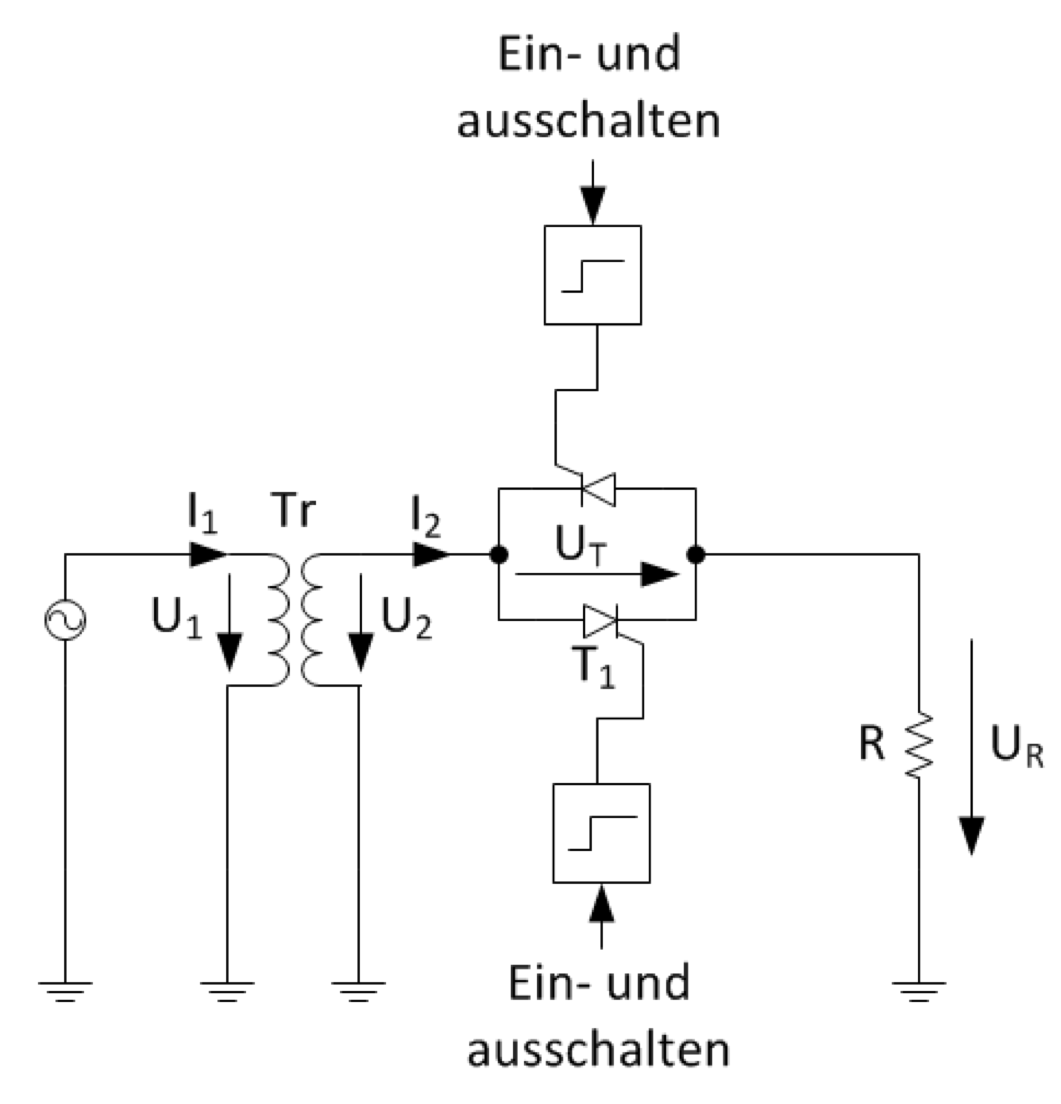
\includegraphics[width=0.85\linewidth]{images/Wechselstromschalter.png}
\end{center}
Ein Wechselstromschalter dient zum reinen \textbf{Ein- und Ausschalten} einer Wechselspannung.
Es findet \textbf{keine Stellfunktion} statt.

Eigenschaften:
\begin{itemize}
    \item Steuerung: Ein/Aus
    \item Keine Spannungsformänderung
    \item Typische Bauelemente: Relais, Triac, antiparallele Thyristoren
\end{itemize}

\crd{\textrightarrow\ Wechselstromschalter sind keine Steller.}

% -------------------------------------------------

\subsection{Wechselstromsteller (Phasenanschnittsteller)}

% --- bestehende Grafik: Phasenanschnitt ---
Phasenanschnittsteuerung beim Wechselstromsteller
\begin{center}
    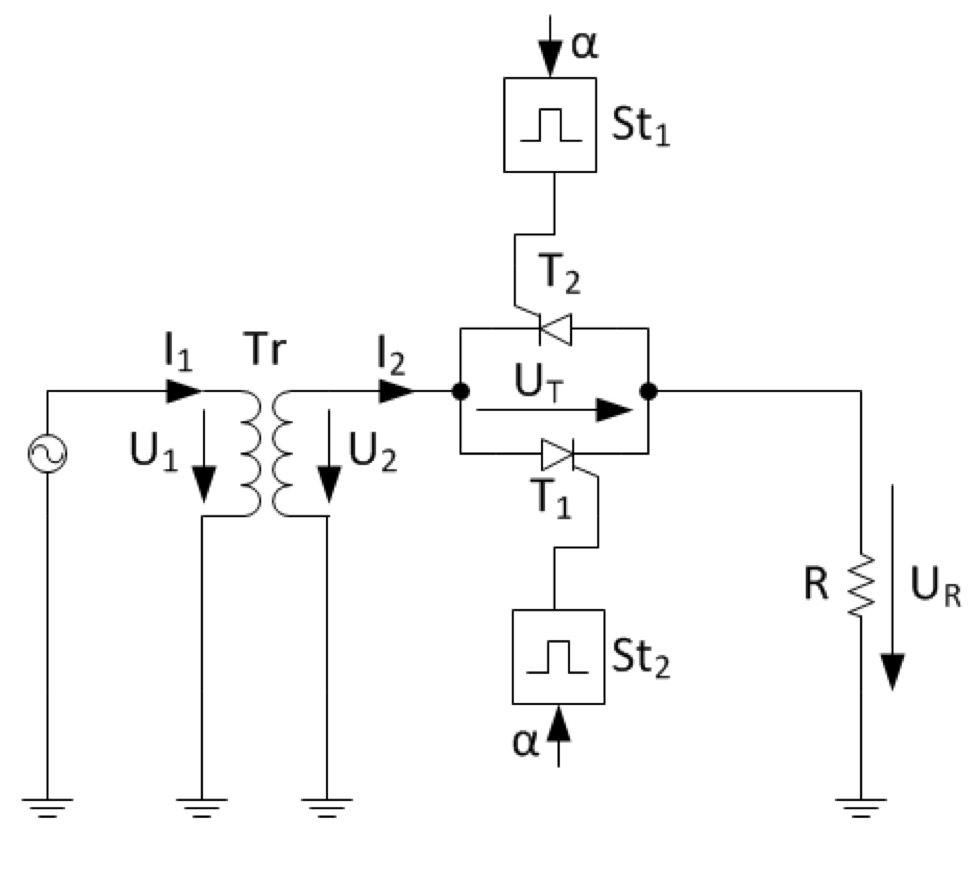
\includegraphics[width=0.85\linewidth]{images/Wechselstromsteller.png}
\end{center}

Ein Wechselstromsteller wandelt eine konstante Wechselspannung in eine \textbf{veränderliche Wechselspannung}.
Die Stellgrösse ist der Zündwinkel $\alpha$.

Momentane Ausgangsspannung:
\[
u(t) =
\begin{cases}
u_s(t), & \omega t \ge \alpha \\
0, & \omega t < \alpha
\end{cases}
\]

Effektivwert (R-Last):
\[
\cbl{U_{\mathrm{RMS}}(\alpha) = U \sqrt{\frac{1}{\pi} \int_\alpha^\pi \sin^2\theta \, d\theta}}
\]

\paragraph{Geschlossene Formel für Effektivwert (R-Last)}
\[
U_{\mathrm{RMS}}(\alpha) = U_s \sqrt{\frac{1}{2\pi} \left( \pi - \alpha + \frac{1}{2}\sin 2\alpha \right)}
\]

Eigenschaften:
\begin{itemize}
    \item Stellgrösse: Zündwinkel $\alpha$
    \item Nichtsinusförmige Spannung
    \item Einsatz: Heizung, Lichtdimmer
\end{itemize}

\subsection{Abgrenzung Schalter -- Steller}

\begin{center}
\begin{tabular}{l|c|c}
 & Schalter & Steller \\ \hline
Funktion & Ein/Aus & \cbl{Stellbar} \\
Stellgrösse & keine & Zündwinkel $\alpha$ \\
Spannungsform & unverändert & \cbl{verformt} \\
\end{tabular}
\end{center}
